\newpage
\section{Adversarial attacks}
\label{sec3}

\subsection{Generating and defending against adversarial attacks}

\subsubsection{Nomenclature of attacks}

We have recently seen deep neural networks match or exceed human-level performance in otherwise arduously difficult tasks (e.g. self-driving cars, medical diagnosis, natural language processing) in the early 2010s. At the same time, there has been a growing body of research literature, starting with \cite{Szegedy2014} and \cite{Goodfellow2014}, on how deep neural networks could be crippled by external attacks designed to fool those models into making (seemingly) absurd mistakes. An early infamous example of how easy it is to cripple state-of-the-art neural networks was provided by \cite{Goodfellow2014}: the authors were able to easily fool a (then state-of-the-art) GoogleLeNet architecture into misclassifying a panda for a gibbon by introducing imperceptible pixel changes to the original image (cf. Figure \ref{fig:Adv_001_Fig}).


\vspace{0.2cm}

\begin{figure}[H]
	\centering
	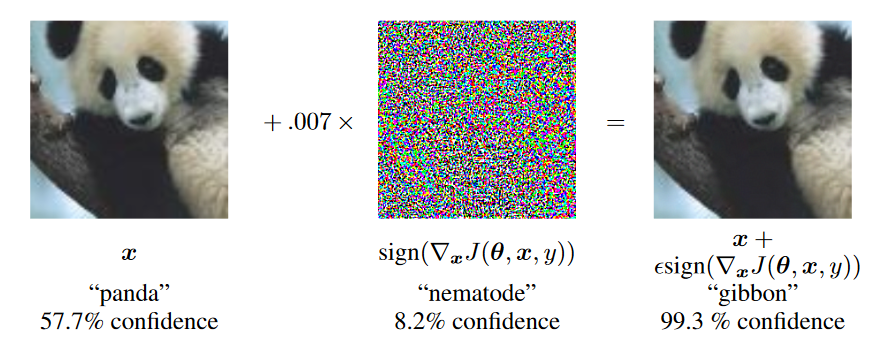
\includegraphics[scale=0.85]{images/adversarial_attacks/Adv_Fig_001_Panda_Picture.PNG}
	\caption{An example of fooling GoogleLeNet into mistaking a panda for a gibbon, source: \cite{Goodfellow2014}}
	\label{fig:Adv_001_Fig}
\end{figure}

\vspace{0.2cm}

Such vulnerabilities constitute a major roadblock for further inroads of AI-Deep Learning-based applications in more critical decision-making fields (e.g. governmental/military applications, more invasive medical procedures). This is further compounded by the ominous nature of adversarial attacks, which the research community is still debating today over its theoretical origins and whether (or not) it is specific to Deep Learning.

The possibility of crippling machine learning algorithms was already a research topic in the early 2000s. But the successes of Deep Learning have further elevated the need for researchers and industry-specialists to tackle the brittleness of machine learning algorithms when deployed outside a closed system where distributional assumptions on the data no longer hold.

As seen in \cite{Nicolae2018AdversarialRT}, there is a distinction between attacks specifically designed to fool neural networks (known as adversarial attacks) and those designed to poison the model's training set thus also crippling the predictive power of neural networks (poisoning attacks). Among adversarial attacks, there is a further demarcation between targeted attacks (where the neural network is fooled into predicting a specific class) and untargeted attacks (fooled into predicting any class). We will mainly focus on untargeted attacks for the remainder of this section. And more importantly, there is an additional distinction between white-box and black-box approaches to generating adversarial attacks.


\subsubsection{White-box and black-box methods}

Assume we are in a multi-classification setting with model image inputs $ x \in \mathbb{R}^{W \times H \times C} $ where $W$, $H$ and $C$ are respectively image width, height and the number of colour channels. The classification of an input $x$ as an output vector $y \in \mathbb{R}^K $ (where $K$ is the number of labels)  is given by a classifier $C$:

$$ C(x) = \arg \max_{y\in \{0,...,K\}} F_y (x) $$

where $F$ is a function that outputs the softmax probabilities for an input image $x$. From there, the most common approach for generating adversarial attacks to fool a specific neural network requires accessing the model's internals: notably the model's cost function $L: X \times Y \rightarrow \mathbb{R} $ such as the cross-entropy function and gradients $\nabla_x L(x,y)$. Once accessed, a wide range of techniques can be used to craft adversarial examples with relatively low complexity.

An early approach for generating adversarial attacks, still used today due to its computational efficiency, is the Fast Gradient Sign Method (FGSM). First introduced by \cite{Goodfellow2014} as a more efficient-version of \cite{Szegedy2014}, it consists in perturbing an image $x^{*}$ labelled $y^{*}$ with an imperceptible perturbation $\psi(x^{*})$. With our human vision, the newly perturbed input $x_{adv}^{*} = x^{*} + \psi(x^{*})$ is still ostensibly the same image as before. But when fed into our classifier, it ends up predicting the wrong class: $C(x^{*} + \psi(x^{*})) \neq y^{*}$. More specifically to FGSM, the adversarial perturbation $\psi(x^{*})$ is crafted by using the model's loss gradients $\nabla_{x^{*}} L(x^{*},y^{*})$ for a given image $x^{*}$:

$$ \psi(x^{*}) = - \varepsilon \cdot \mathbf{sign}(\nabla_{x^{*}} L(x^{*},y^{*})) $$

$$ x_{adv}^{*} = \mathbf{clip}(x + \psi(x^{*}), x_{min}, x_{max} )$$

where $\varepsilon$ is the strength of the attack. Excessive $\varepsilon$ values will make the adversarial attack more noticeable to human observers. The clipping function as well as input bounds $x_{min}$ and $x_{max}$ ensure that the adversarially crafted input remains an image.

There have been alternative white-box approaches for generating adversarial attacks, notably Projected Gradient Descent (PGD), Jacobian Saliency Map Attack (JSMA) or Carlini \& Wagner $L_2$ Attack (C\&W). IBM's Adversarial Robustness Toolbox from \cite{Nicolae2018AdversarialRT} has a wide range of options for crafting more sophisticated white-box adversarial attacks. Nevertheless, due to its computational efficiency, FGSM remains a popular technique for applications that require generating a large set of adversarial examples (notably adversarial training as we will see in a later subsection).

One notable weakness of white-box methods for targeting deep neural networks is that they require accessing the network's internals (notably gradients). Since \cite{Papernot2017PracticalBA}, black-box methods for fooling deep neural networks were devised, requiring neither access to the model architecture or the original training set used to train the targeted model. Examples include using substitute models mimicking the targeted classifier for crafting adversarial examples, Zeroth-Order Optimization or HopSkipJump Attack. These techniques exploit the transferability property of adversarial attacks (which will be further explored in the next section) and have shown high attack success rates against state-of-the-art architectures as seen in \cite{Papernot2017PracticalBA} and \cite{Chen2017ZOOZO}.


\subsubsection{Defences against adversarial attacks}

Machine Learning researchers have devoted a lot of time and effort on devising effective counter-measures for protecting neural networks from adversarial attacks. They broadly fall into three main categories:

\begin{itemize}
	\item \textbf{Adversarial Training}: one of the earliest defence strategies is introducing adversarial examples into the training phase, generated from the initial training data. The authors \cite{Szegedy2014} and \cite{Goodfellow2014} who brought the existence of adversarial attacks to the attention of the research community proposed adversarial training as an easily implementable approach for hardening classifiers against adversarial attacks. For generating adversarial examples, FGSM is the preferred approach due its low computational complexity.
	\item \textbf{Image Squeezing}: as detailed in \cite{Nicolae2018AdversarialRT}, there exists a number of compression techniques (such as JPEG or thermometer compression) for blurring images, therefore reducing the magnitude of adversarial perturbations. \cite{Shafahi2018} provides a theoretical justification in that blurring images reduces image complexity thus leading to a classifier with a more concentrated image distribution making it more robustness to attacks.
	\item \textbf{Anomaly Detection}: this approach augments the existing classifier to help detect whether an incoming image is an adversarial example or not. One of the more complex attempts from \cite{Samangouei2018DefenseGANPC} to dampen the magnitude of adversarial attacks is to "project" input images into a separately-trained Generative Adversarial Network (GAN) and feed the GAN's output into the classifier rather than the original image.
\end{itemize}


Despite the proliferation of defensive strategies, as pointed out by \cite{Shafahi2018}, many of those techniques have almost been immediately broken. Most of these approaches are only suited for shielding neural networks against a specific type of attack (e.g. white-box, black-box), e.g. adversarial training with FGSM can be easily circumvented with more advanced black-box attacks.



\subsection{Why study adversarial attacks?}

\subsubsection{Existence and transferability of adversarial attacks}

The existence and inevitability of adversarial attacks have been a major research topic within the Machine Learning research community since \cite{Szegedy2014} and \cite{Goodfellow2014}.

One of the earliest explanations for the puzzling behaviour of adversarial attacks was provided by \cite{Goodfellow2014} as the "linear hypothesis". Suppose we start in the linear case and we make small additive perturbations to an input image such that $\tilde x = x + \eta $, our classifier will yield the following output:

$$ w^T \tilde x = w^T x + w^T \eta $$

If this additive perturbation is small enough, where $\Vert \eta \Vert_{\infty} \leq \epsilon$, then it would not make sense for the classifier to react differently (i.e. predict a different label). We can see that there is a linear relationship between our perturbation and its effect on our classifier $ w^T \eta $.

But as \cite{Goodfellow2014} points out, increasing the complexity of the images we are dealing with (e.g. moving from greyscale to RGB) also simultaneously increases (linearly) the damage those perturbations can wreck on our classifier. This comes from the fact that the more complex our image becomes, more and more pixels become available to be fooled around. Thus, it becomes easier to make imperceptible input changes on larger swaths of our image (such that the image still looks broadly the same as before since $\Vert \eta \Vert_{\infty} \leq \epsilon$). The  higher the dimensionality of our targeted image is, the more potent the perturbations $ w^T \eta $ will be on our classifier. While this explanation was elaborated for linear models, \cite{Goodfellow2014} claims that this also holds true for neural networks. Neural networks in multi-class classification by construction use softmax regression for making predictions, which is in itself a generalization of logistic regression - a linear model.


The high-dimensionality of images has thus been the preferred explanation for the continued existence of adversarial attacks. As pointed out by \cite{shafahi2018adversarial}, many studies have shown that state-of-the-art neural networks are more easily fooled on RGB datasets (e.g. CIFAR-10, ImageNet) than on grey scaled datasets (e.g. MNIST).

While there have been numerous hints that the high-dimensionality of RGB image datasets might be the root cause of adversarial attacks, \cite{shafahi2018adversarial} have shown that dimensionality is not necessarily by itself the main driver behind the ease of crafting attacks to fool neural networks or even the failure of many adversarial defensive strategies. They created an upscaled version of MNIST with higher resolution grey scaled images of shape $56 \times 56$ ($b$-MNIST) and test the robustness of different neural networks on MNIST, $b$-MNIST and CIFAR-10. Even though $b$-MNIST roughly has the same pixel complexity as CIFAR-10, the adversarial robustness on $b$-MNIST is roughly the same as with MNIST thus noticeably higher than with CIFAR-10 models.


For the authors, input concentration - specifically how diversely distributed the images are in input space - is likely to play a more important role than dimensionality alone. This ties smoothly with their finding that the success rate of adversarial attacks stems primarily from how concentrated the input image space is: classifiers trained on highly-concentrated image data will be more robustness to adversarial attacks. The MNIST dataset is highly concentrated since images tend to roughly have the same profile: centred grey-scaled digits. Thus, upscaling MNIST wouldn't lead to changes in input image distribution thus adversarial robustness would not change in anyway. Conversely, CIFAR-10 has lower data concentration due to higher image complexity. Theoretically, this should increase the successfulness of adversarial attacks (which is confirmed in the case of MNIST-trained classifiers being more adversarially robust than CIFAR-10 or ImageNet classfiers).


Another intriguing property of adversarial examples is their transferability. \cite{moosavidezfooli2016universal} showed a rather disconcerting result. It is possible for a specific neural architecture (e.g. VGG16, Inception, ResNet) to craft model-specific perturbations that will succeed in defeating the said architecture all the time, regardless of the dataset. They have even shown these examples can also transfer between model architectures. These are known as universal adversarial attacks.



\vspace{0.2cm}

\begin{figure}[H]
	\centering
	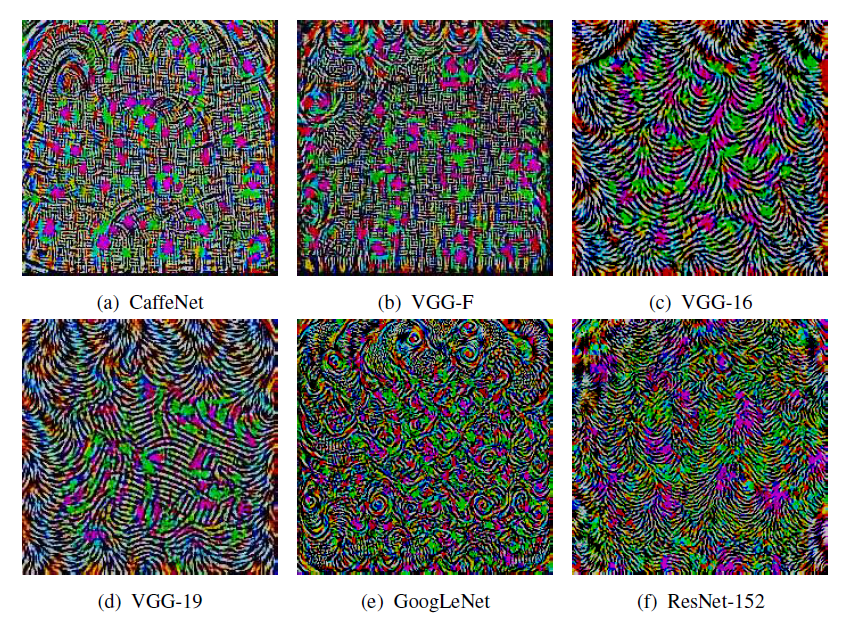
\includegraphics[scale=0.85]{images/adversarial_attacks/Adv_Fig_002_UAE.PNG}
	\caption{Universal adversarial attacks for different state-of-the-art classifiers, source: \cite{moosavidezfooli2016universal}}
	\label{fig:Adv_002_Fig}
\end{figure}

\vspace{0.2cm}


\subsubsection{Vulnerabilities in real-world conditions}

Even though adversarial attacks have bore the focus of the research community since the 2010s, there exists another type of vulnerability that has seen less attention but is likely to happen more often than not in a real-world environment: corruption robustness (e.g. brightness changes, blur, pixelation, anomalous objects disrupting images, random rotations). According to \cite{ford2019adversarial}, at first adversarial attacks and corruption vulnerabilities are seemly unrelated, but in reality it turns out to be opposite.

\vspace{0.2cm}


\begin{figure}[H]
	\centering
	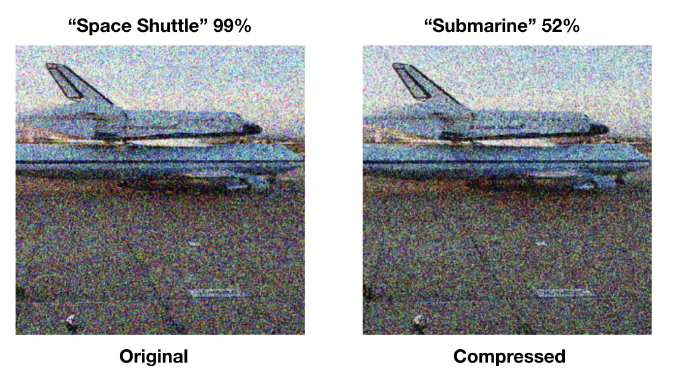
\includegraphics[scale=0.85]{images/adversarial_attacks/Adv_Fig_003_Gaussian_Noise.PNG}
	\caption{Corruption robustness on ImageNet after adding Gaussian noise, source: \cite{ford2019adversarial}}
	\label{fig:Adv_003_Fig}
\end{figure}

\vspace{0.2cm}

\cite{ford2019adversarial} show (theoretically) on linear models that adversarially generated examples lie on the same high dimensional image space as images generated with additive Gaussian random perturbations. They extend their initial results to neural networks by running a number of experiments on CIFAR-10 and ImageNet. From a distributional perspective, adversarial attacks and corruption vulnerabilities emanate from the same underlying manifold.

Self-driving cars are an example of a field where the consequences of adversarial attacks could be particularly severe. While brittleness to blurred/corrupted video planes is most likely to be the most obvious threat for self-driving cars, \cite{Ranjan2019AttackingOF} have shown that targeted attacks (e.g. adversarial image patches that amount to less than 1\% of the total video frame) can compromise video streams and consequently self-driving cars.

\vspace{0.2cm}


\begin{figure}[H]
	\centering
	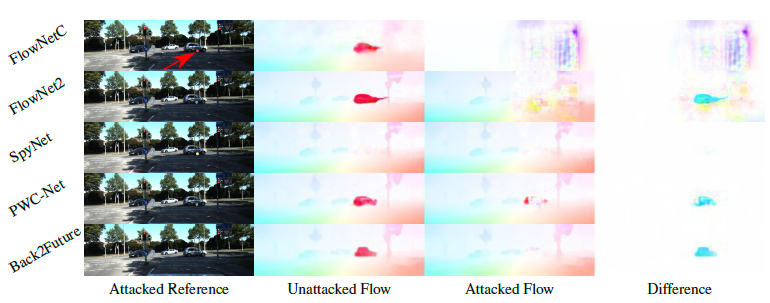
\includegraphics[scale=0.94]{images/adversarial_attacks/Adv_Fig_004_Self_Driving_Cars.PNG}
	\caption{Adversarial patches on video streams, source: \cite{Ranjan2019AttackingOF}}
	\label{fig:Adv_004_Fig}
\end{figure}

\vspace{0.2cm}

Another novel playground for adversarial attacks is fooling deepfake detectors. Concern over the dangerousness of deepfakes in spreading disinformation has led tech giants such as Facebook and Twitter to develop deepfake detectors. In February 2020, Kaggle even hosted a DeepFake detection competition with the blessing of major tech companies such as Amazon, Microsoft and Facebook. But more recent studies from \cite{Neekhara2020AdversarialDE} and \cite{Gandhi2020AdversarialPF} have shown that deepfake detectors can be easily fooled by even the simplest methods such as FGSM.


\subsubsection{Is there a trade-off between robustness and generalization?}

A more pressing concern is whether improving the robustness of classifiers against adversarial attacks necessarily leads to a trade-off in performance. Popular adversarial defences such as adversarial training introduce adversarially generated examples during backpropagation, which could theoretically diminish predictive performance on newer images.

\cite{tsipras2018robustness} found that there exists effectively an empirically-observable trade-off between robustness to adversarial attacks and testing set performance as seen on Figure \ref{fig:Adv_005_Fig}. The drop in performance is slightly more pronounced on CIFAR-10.

\vspace{0.2cm}

\begin{figure}[H]
	\centering
	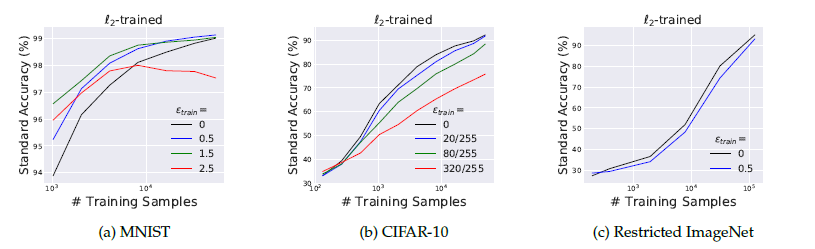
\includegraphics[scale=1.0]{images/adversarial_attacks/Adv_Fig_005_Robustness_1.PNG}
	\caption{Trade-off between adversarial robustness and testing set accuracy on adversarially trained classifiers, source: \cite{tsipras2018robustness}}
	\label{fig:Adv_005_Fig}
\end{figure}

\vspace{0.2cm}

Yet in spite of this empirical trade-off, they found that there was an unexpected silver lining in adversarially training neural networks: they ran a number of interpretability diagnostics with saliency maps in order to understand the decision-making process of neural networks (as showcased on Figure \ref{fig:Adv_006_Fig}). They found that adversarially trained neural networks did a much better job in localizing the relevant object compared to standard non-robust neural networks and thus were more semantically aligned with our human visual stream than the latter.


\vspace{0.2cm}

\begin{figure}[H]
	\centering
	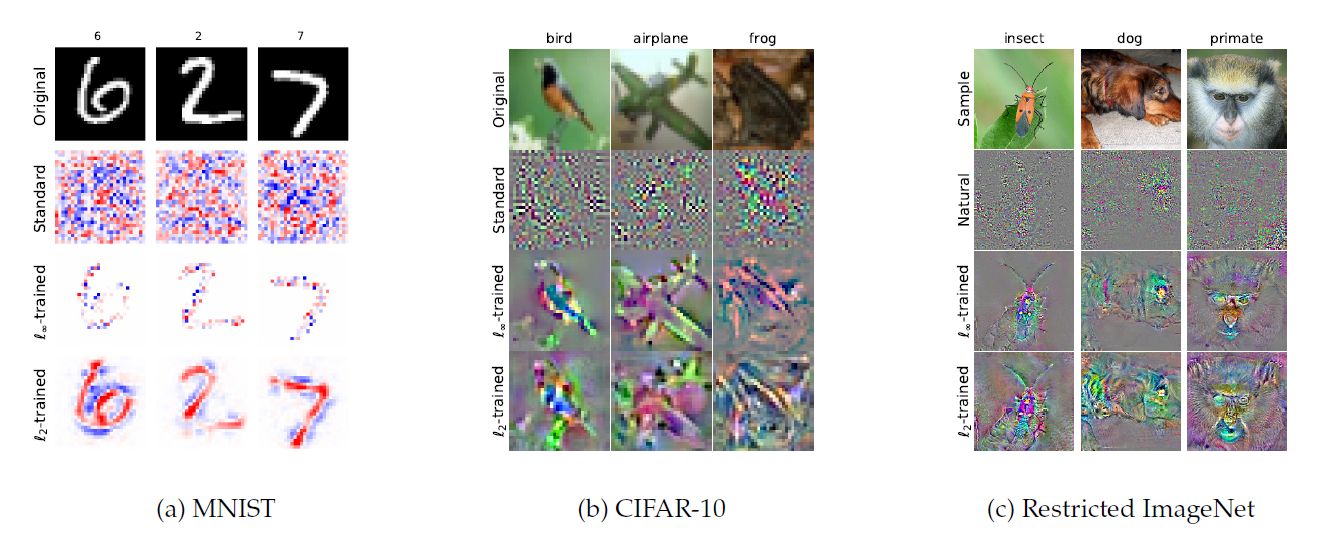
\includegraphics[scale=0.6]{images/adversarial_attacks/Adv_Fig_006_Robustness_2.PNG}
	\caption{Saliency maps on non-robust and $L_2$-adversarially trained neural networks, source: \cite{tsipras2018robustness}}
	\label{fig:Adv_006_Fig}
\end{figure}

\vspace{0.2cm}

Therefore, adversarial robustness improves model interpretability and brings black-box neural networks closer to human vision. Notably, by preventing the latter from concentrating undue attention on non-robust features and instead focus on the image contours/ensembles that would really matter when attempting to localize objects on an image.

\subsection{Adversarial robustness simulator with Plotly Dash}

To illustrate our literature review, we developed an adversarial attack simulator for stress testing Keras models. It is actually a sub-component of much larger interpretability framework - \textbf{Deep Embedding Viewer} - that we will go into greater detail later.

After selecting an available Keras model, the user can run a series of adversarial pertrubations to stress test the model's adversarial robustness. For this application, we chose to generate adversarial attacks with the FGSM method due to its low complexity and our need to generate many adversarial samples.

Once the "Run Stress Test" switch is pressed, FGSM perturbations are added to the classifier's validation/testing set. Different perturbations levels $\varepsilon$ are considered from 0.5\% to 10\%: in an ideal outcome, our neural network should be robust to attacks with low perturbation levels (e.g. 0.5\%, 1\% and 2.5\%) as at this stage the perturbations are imperceptible to an human observer.

We demonstrate the use of our simulator on a VGG-16 model trained on CIFAR-10 and evaluated on a validation set of 10,000 images. Once the simulation generated 10,000 adversarial images a performance chart is displayed (on the left in Figure \ref{fig:Adv_007_Fig}), summarizing the adversarial robustness of our classifier against different perturbation scenarios. On the right, a slider is provided to visualize concretely different perturbation $\varepsilon$ values and help the user get a better sense of how adversarial attacks discretely distort images.


\vspace{0.2cm}

\begin{figure}[H]
	\centering
	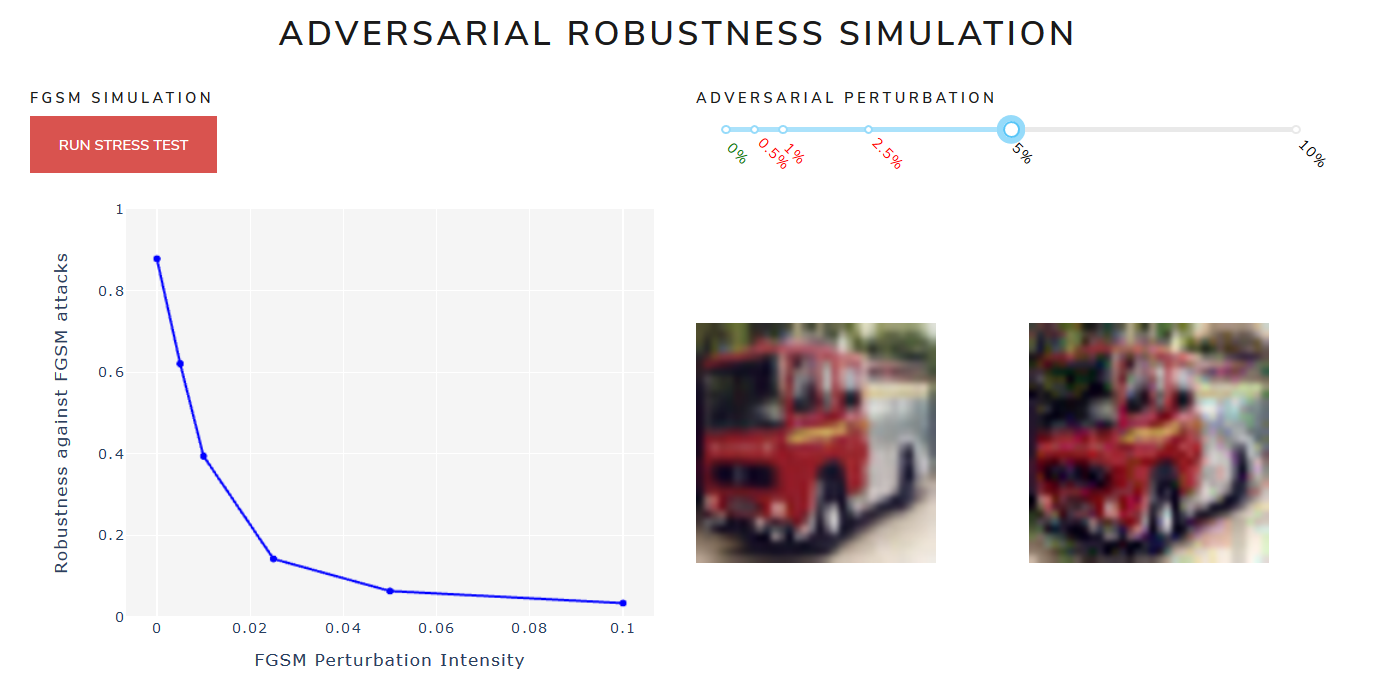
\includegraphics[scale=0.65]{images/adversarial_attacks/Adv_Fig_007_Simulator.PNG}
	\caption{Adversarial Robustness Simulator (with FGSM) for Keras Models}
	\label{fig:Adv_007_Fig}
\end{figure}

\vspace{0.2cm}



\newpage